\documentclass[11pt]{article}

\usepackage[T1]{fontenc}
\usepackage[utf8]{inputenc}
\usepackage{lmodern}
\usepackage[margin=1in]{geometry}
\usepackage{microtype}
\usepackage{amsmath,amssymb}
\usepackage{booktabs}
\usepackage{graphicx}
\usepackage{xcolor}
\usepackage{tikz}
\usepackage[round,authoryear]{natbib}
\usepackage[font=small,labelfont=bf]{caption}
\usepackage{enumitem}
\usepackage{float}
\usepackage[colorlinks=true,linkcolor=black!70!blue,citecolor=black!70!blue,urlcolor=black!70!blue]{hyperref}
\usepackage[capitalise,noabbrev]{cleveref}

\definecolor{rmsblue}{HTML}{2A78D6}
\definecolor{taperorange}{HTML}{EB6834}
\definecolor{inkmuted}{HTML}{52514E}
\newcommand{\authornote}[1]{\textcolor{red!70!black}{[\textbf{Author:} #1]}}

% Generated by paper/make_assets.py from reports/h1-kaggle and reports/s2-kaggle -- do not edit by hand.
\newcommand{\Dmean}{\ensuremath{-0.0223}}
\newcommand{\Dsd}{\ensuremath{0.0034}}
\newcommand{\Dlo}{\ensuremath{-0.0308}}
\newcommand{\Dhi}{\ensuremath{-0.0139}}
\newcommand{\Dmin}{\ensuremath{-0.0262}}
\newcommand{\Dmax}{\ensuremath{-0.0200}}
\newcommand{\DthreeMean}{\ensuremath{{+}0.0059}}
\newcommand{\DoneMean}{\ensuremath{{+}0.0102}}
\newcommand{\Qmean}{\ensuremath{-0.0204}}
\newcommand{\Gmean}{\ensuremath{-0.0019}}
\newcommand{\matchedMean}{\ensuremath{-0.0259}}
\newcommand{\matchedTarget}{6{,}104}
\newcommand{\FcodeMin}{\ensuremath{1.63}}
\newcommand{\FcodeMax}{\ensuremath{1.69}}
\newcommand{\FcodeMean}{\ensuremath{1.66}}
\newcommand{\FwebMin}{\ensuremath{-0.128}}
\newcommand{\FwebMax}{\ensuremath{-0.122}}
\newcommand{\DrelPct}{1.3}
\newcommand{\gapMin}{0.28}
\newcommand{\gapMax}{0.34}
\newcommand{\adaptMin}{3.34}
\newcommand{\adaptMax}{3.60}
\newcommand{\earlyMax}{\ensuremath{{+}0.015}}
\newcommand{\earlyMaxAt}{400}
\newcommand{\clipRMSlo}{52}
\newcommand{\clipRMShi}{60}
\newcommand{\clipTaperlo}{61}
\newcommand{\clipTaperhi}{70}
\newcommand{\overflowRetries}{0}
\newcommand{\secRMS}{0.37}
\newcommand{\secTaper}{0.37}
\newcommand{\sessionHours}{9.36}
\newcommand{\sessionStartTime}{12:18}
\newcommand{\sessionEndTime}{21:40}
\newcommand{\sessionStart}{3 October 2026{,} 12:18}
\newcommand{\sessionEnd}{3 October 2026{,} 21:40}
\newcommand{\torchVersion}{2.11.0}
\newcommand{\cudaVersion}{12.8}
\newcommand{\paramsRMS}{17{,}718{,}784}
\newcommand{\paramsTaper}{17{,}721{,}856}
\newcommand{\embedShare}{73}
\newcommand{\nDocsWeb}{4{,}409}
\newcommand{\medianDocMin}{\ensuremath{-0.027}}
\newcommand{\medianDocMax}{\ensuremath{-0.023}}
\newcommand{\configSha}{c18441799eee2b6a}
\newcommand{\runnerSha}{66769e7de30ec36f}
\newcommand{\nearRemoved}{2{,}182}
\newcommand{\exactRemoved}{0}
\newcommand{\repoGroups}{140{,}195}
\newcommand{\auditPairs}{2{,}043}
\newcommand{\auditFound}{0}
\newcommand{\webTrainTokens}{260{,}000{,}257}
\newcommand{\pyTrainTokens}{110{,}000{,}129}
\newcommand{\cfourRev}{1588ec454efa}
\newcommand{\stackRev}{17cad72c886a}
\newcommand{\slopeRMS}{\ensuremath{-0.00244}}
\newcommand{\slopeTaper}{\ensuremath{-0.00249}}
\newcommand{\maxJump}{\ensuremath{0.045}}
\newcommand{\classAneg}{3}
\newcommand{\classAlargest}{2}
\newcommand{\matchedEarlier}{9}
\newcommand{\matchedPairs}{9}
\newcommand{\trajMin}{\ensuremath{-0.024}}
\newcommand{\trajMinAt}{5{,}795}
\newcommand{\trajMax}{\ensuremath{{+}0.024}}
\newcommand{\trajMaxAt}{2{,}745}
\newcommand{\seedAbsMax}{\ensuremath{0.041}}
\newcommand{\nNegEnd}{3}
\newcommand{\DA}{\ensuremath{-0.0200}}
\newcommand{\DoneFiveA}{\ensuremath{{+}0.037}}
\newcommand{\DB}{\ensuremath{-0.0207}}
\newcommand{\DoneFiveB}{\ensuremath{{+}0.022}}
\newcommand{\DC}{\ensuremath{-0.0262}}
\newcommand{\DoneFiveC}{\ensuremath{-0.029}}
\newcommand{\logConfigTime}{12:19:23}
\newcommand{\seedOneFirst}{14:25}
\newcommand{\seedOneLast}{15:26}
\newcommand{\commitTime}{16:07}
\newcommand{\thresholdLine}{82}
\newcommand{\clipBranchLo}{88}
\newcommand{\clipBranchHi}{96}
\newcommand{\clipGateZeroRMS}{15}
\newcommand{\clipGateZeroTaper}{50}
\newcommand{\clipEarlyHi}{16}
\newcommand{\clipCalib}{16}
\newcommand{\clipDecayRMS}{4}
\newcommand{\clipDecayTaper}{11}
\newcommand{\maxLossScale}{16{,}384}
\newcommand{\earlyLo}{\ensuremath{-0.0185}}
\newcommand{\earlyHi}{\ensuremath{-0.0130}}
\newcommand{\midMean}{\ensuremath{{+}0.002}}
\newcommand{\midMin}{\ensuremath{-0.012}}
\newcommand{\midMax}{\ensuremath{{+}0.024}}
\newcommand{\midCount}{15}
\newcommand{\lateMean}{\ensuremath{-0.020}}
\newcommand{\lateCount}{5}
\newcommand{\midSD}{\ensuremath{0.0164}}
\newcommand{\finalSD}{\ensuremath{0.0034}}
\newcommand{\sdRatio}{4.8}
\newcommand{\lateLRpct}{9}
\newcommand{\lateNeg}{5}
\newcommand{\lateNegSeedPoints}{15}
\newcommand{\lateSeedPoints}{15}
\newcommand{\dipMean}{\ensuremath{-0.0185}}
\newcommand{\dipSD}{\ensuremath{0.0021}}
\newcommand{\Rlabels}{5{,}147--5{,}285}
\newcommand{\RmeanLo}{\ensuremath{-0.206}}
\newcommand{\RmeanHi}{\ensuremath{-0.082}}
\newcommand{\RcontribLo}{\ensuremath{-0.0005}}
\newcommand{\RcontribHi}{\ensuremath{-0.0002}}
\newcommand{\RsharePct}{3}
\newcommand{\bootB}{10{,}000}
\newcommand{\bootLo}{\ensuremath{-0.0235}}
\newcommand{\bootHi}{\ensuremath{-0.0211}}
\newcommand{\bootSE}{\ensuremath{0.0006}}
\newcommand{\bootSeedSElo}{\ensuremath{0.0009}}
\newcommand{\bootSeedSEhi}{\ensuremath{0.0010}}
\newcommand{\bootRatioSeed}{3.6}
\newcommand{\seedSEmean}{\ensuremath{0.0020}}
\newcommand{\bootRatioMean}{3.3}
\newcommand{\scaleGapR}{0.097}
\newcommand{\scaleGapPctR}{10}
\newcommand{\scaleWebAbsR}{0.206}
\newcommand{\scalePyAbsR}{0.207}
\newcommand{\scaleWebSignedR}{\ensuremath{-0.206}}
\newcommand{\scalePySignedR}{\ensuremath{-0.196}}
\newcommand{\scaleWebFactorR}{0.81}
\newcommand{\scalePyFactorR}{0.82}
\newcommand{\scaleSpecificR}{0.042}
\newcommand{\scaleSpecificPctR}{4}
\newcommand{\scaleWebShrinkR}{36}
\newcommand{\scalePyShrinkR}{30}
\newcommand{\scaleGapT}{0.123}
\newcommand{\scaleGapPctT}{13}
\newcommand{\scaleWebAbsT}{0.054}
\newcommand{\scalePyAbsT}{0.077}
\newcommand{\scaleWebSignedT}{\ensuremath{{+}0.040}}
\newcommand{\scalePySignedT}{\ensuremath{{+}0.060}}
\newcommand{\scaleWebFactorT}{1.04}
\newcommand{\scalePyFactorT}{1.06}
\newcommand{\scaleSpecificT}{0.042}
\newcommand{\scaleSpecificPctT}{4}
\newcommand{\scaleWebShrinkT}{6}
\newcommand{\scalePyShrinkT}{3}
\newcommand{\scalePairs}{36}
\newcommand{\lshMiss}{\ensuremath{5.5\times10^{-11}}}
\newcommand{\lshRecallSeventy}{0.9998}
\newcommand{\shortDocs}{20}
\newcommand{\twoSelZh}{0.0934}
\newcommand{\twoSelRu}{0.0893}
\newcommand{\twoSelDe}{0.0514}
\newcommand{\twoSelOwm}{0.0119}
\newcommand{\twoSelPy}{0.1099}
\newcommand{\twoSelPyR}{0.0971}
\newcommand{\twoSelPyT}{0.1228}
\newcommand{\twoReproMax}{0.0}
\newcommand{\twoTrainTokens}{110{,}000{,}129}
\newcommand{\twoTrainDocs}{56{,}276}
\newcommand{\twoDevDocs}{1{,}139}
\newcommand{\twoTestDocs}{4{,}201}
\newcommand{\twoNearRemoved}{698}
\newcommand{\twoExactRemoved}{0}
\newcommand{\twoFrozenRemoved}{0}
\newcommand{\twoAuditPairs}{2{,}443}
\newcommand{\twoFrozenPairs}{2{,}000}
\newcommand{\twoTrainShards}{2}
\newcommand{\twoValShards}{1}
\newcommand{\twoRawTrain}{126.5}
\newcommand{\twoSessOne}{11.12}
\newcommand{\twoSessTwo}{4.06}
\newcommand{\twoSessTotal}{15.17}
\newcommand{\twoTorch}{2.11.0}
\newcommand{\twoManifestSha}{3eeda992819a}
\newcommand{\twoSubmit}{21:55 UTC on 8 October}
\newcommand{\twoFirstJob}{21:56 UTC on 8 October}
\newcommand{\twoRunStart}{22:59 UTC on 8 October}
\newcommand{\twoBlock}{970{,}569}
\newcommand{\twoBlockTime}{01:59 UTC on 9 October}
\newcommand{\twoBlockAfterStart}{3}
\newcommand{\twoLineageN}{24}
\newcommand{\twoSecRMS}{0.37}
\newcommand{\twoSecTaper}{0.37}
\newcommand{\twoClipXR}{99.5}
\newcommand{\twoClipXT}{99.7}
\newcommand{\twoClipPyR}{94}
\newcommand{\twoClipWebR}{90}
\newcommand{\twoDmean}{\ensuremath{-0.0325}}
\newcommand{\twoDsd}{\ensuremath{0.0341}}
\newcommand{\twoDlo}{\ensuremath{-0.0683}}
\newcommand{\twoDhi}{\ensuremath{{+}0.0032}}
\newcommand{\twoDloNinety}{\ensuremath{-0.0606}}
\newcommand{\twoDhiNinety}{\ensuremath{-0.0045}}
\newcommand{\twoDmin}{\ensuremath{-0.0886}}
\newcommand{\twoDmax}{\ensuremath{{+}0.0065}}
\newcommand{\twoNneg}{5}
\newcommand{\twoPosSeed}{102}
\newcommand{\twoPosD}{\ensuremath{{+}0.0065}}
\newcommand{\twoDthree}{\ensuremath{-0.0338}}
\newcommand{\twoQmean}{\ensuremath{-0.0306}}
\newcommand{\twoGmean}{\ensuremath{-0.0019}}
\newcommand{\twoMatched}{\ensuremath{-0.0378}}
\newcommand{\twoMatchedTarget}{6{,}104}
\newcommand{\twoGapMin}{0.23}
\newcommand{\twoGapMax}{0.34}
\newcommand{\twoAdaptMin}{2.18}
\newcommand{\twoAdaptMax}{2.33}
\newcommand{\twoFxMin}{\ensuremath{2.34}}
\newcommand{\twoFxMax}{\ensuremath{2.55}}
\newcommand{\twoFxMean}{\ensuremath{2.41}}
\newcommand{\twoDrelPct}{1.3}
\newcommand{\twoFreshMean}{\ensuremath{-0.0260}}
\newcommand{\twoFreshLo}{\ensuremath{-0.0816}}
\newcommand{\twoFreshHi}{\ensuremath{{+}0.0296}}
\newcommand{\twoBootLo}{\ensuremath{-0.0339}}
\newcommand{\twoBootHi}{\ensuremath{-0.0311}}
\newcommand{\twoEarlyMax}{\ensuremath{{+}0.012}}
\newcommand{\twoEarlyMaxAt}{650}
\newcommand{\twoTrajNeg}{22}
\newcommand{\twoTrajN}{24}
\newcommand{\twoMedianMin}{\ensuremath{-0.064}}
\newcommand{\twoMedianMax}{\ensuremath{{+}0.010}}
\newcommand{\twoMedianNeg}{5}
\newcommand{\twoLateMean}{\ensuremath{-0.0237}}
\newcommand{\twoLateNeg}{5}
\newcommand{\twoLateCount}{5}
\newcommand{\twoJitter}{\ensuremath{0.040}}
\newcommand{\twoCtrlShare}{85}
\newcommand{\webCtrlShare}{2.2}
\newcommand{\twoPrefixCE}{4.58}
\newcommand{\twoWebEndCE}{4.46}
\newcommand{\twoXendCE}{6.99}
\newcommand{\twoOverflow}{0}
\newcommand{\twoClassPneg}{5}
\newcommand{\twoClassAneg}{4}
\newcommand{\twoRareMax}{0.0007}
\newcommand{\twoSdRatio}{10}
\newcommand{\repInPilot}{0}
\newcommand{\repDmean}{\ensuremath{{+}0.0093}}
\newcommand{\repDsd}{\ensuremath{0.0071}}
\newcommand{\repDlo}{\ensuremath{-0.0084}}
\newcommand{\repDhi}{\ensuremath{{+}0.0271}}
\newcommand{\repDloNinety}{\ensuremath{-0.0027}}
\newcommand{\repDhiNinety}{\ensuremath{{+}0.0214}}
\newcommand{\repDvalues}{\ensuremath{{+}0.0160}{,} \ensuremath{{+}0.0102}{,} \ensuremath{{+}0.0018}}
\newcommand{\repNpos}{3}
\newcommand{\repDthree}{\ensuremath{{+}0.0042}}
\newcommand{\repQmean}{\ensuremath{{+}0.0113}}
\newcommand{\repMatched}{\ensuremath{{+}0.0174}}
\newcommand{\repGapMin}{0.23}
\newcommand{\repGapMax}{0.30}
\newcommand{\repAdaptMin}{3.38}
\newcommand{\repAdaptMax}{3.64}
\newcommand{\poolMean}{\ensuremath{-0.0065}}
\newcommand{\poolSd}{\ensuremath{0.0180}}
\newcommand{\poolLo}{\ensuremath{-0.0254}}
\newcommand{\poolHi}{\ensuremath{{+}0.0125}}
\newcommand{\poolSdRatio}{5}
\newcommand{\mcGapXR}{0.085}
\newcommand{\mcGapXT}{0.122}
\newcommand{\mcGapPyR}{0.093}
\newcommand{\mcGapPyT}{0.136}
\newcommand{\mcSpecXR}{0.165}
\newcommand{\mcSpecXT}{0.183}
\newcommand{\mcSpecPyR}{0.039}
\newcommand{\mcSpecPyT}{0.042}
\newcommand{\mcRatioLo}{4.3}
\newcommand{\mcRatioHi}{4.4}
\newcommand{\mcXfactorR}{0.72}
\newcommand{\mcXfactorT}{1.21}
\newcommand{\mcWebFactorR}{0.82}
\newcommand{\mcWebFactorT}{1.05}


\title{No Evidence That TaperNorm Increases Forgetting After a Web-to-Code Domain Shift:\\ A Pre-Specified Pilot Study}
\author{\authornote{Author name}\\ \authornote{Affiliation, or ``Independent researcher''}\\ \authornote{email}}
\date{First draft --- not for distribution}

\begin{document}
\maketitle

\begin{abstract}
TaperNorm \citep{kanavalau2026tapernorm} replaces the internal normalization layers of a pre-norm Transformer
with a gated map that behaves like RMSNorm early in training and then tapers to a fixed, calibrated,
sample-independent scaling. A tapered layer no longer rescales each token by its own statistics, which raises a
natural concern: such a model might forget more when its training distribution shifts. We tested this concern
in a small pilot whose design, primary endpoint and decision rules were specified before training.
Small decoder-only language models (17.7M parameters), using either internal RMSNorm or internal TaperNorm,
were trained on 150M tokens of web text (C4). Each was then continued for 100M tokens either on further web text
or on Python code (The Stack), with three paired seeds. The primary endpoint is a difference-in-differences $D$ of
held-out web cross-entropy, where positive values mean more excess forgetting under TaperNorm. Switching to
Python raised web cross-entropy by about \FcodeMean{}~nats/token in both conditions. Mean $D$ was \Dmean{}~nats/token
(seeds \DA, \DB, \DC), which is below the pre-specified $+0.015$ bound for a meaningful excess.
The pre-specified decision is therefore to stop: we find no evidence that TaperNorm increases persistent
forgetting in this setting. The endpoint difference points the opposite way in all three seeds, but it is small,
it falls short of the pre-specified threshold for an opposite-direction effect, and the seed-mean contrast varied
between \trajMin{} and \trajMax{} across intermediate checkpoints, so we do not claim that TaperNorm reduces
forgetting. Code, the frozen configuration and all evaluation records are released.
\end{abstract}

\section{Introduction}

Normalization layers such as LayerNorm \citep{ba2016layer} and RMSNorm \citep{zhang2019rmsnorm} are a standard
part of Transformer language models. In the common pre-norm arrangement \citep{xiong2020layer}, every attention
and MLP sub-layer reads its input through a normalizer that rescales each token's activation vector by that
token's own statistics. A long line of work has asked whether normalization is necessary at all
\citep{zhang2019fixup,brock2021nfnet}. TaperNorm \citep{kanavalau2026tapernorm} is a recent proposal for
Transformers. It acts exactly as RMSNorm (or LayerNorm) during an initial gate warm-up, calibrates a fixed
scaling branch during that warm-up, and then cosine-decays a global gate until each internal normalizer becomes
a sample-independent linear map. That map can be folded into the adjacent linear projections at inference.
\citet{kanavalau2026tapernorm} report that this matches normalized baselines under identical setups, and they
measure up to $1.22\times$ higher throughput in an inference microbenchmark.

This study looks at a property that the original evaluation did not target: behaviour under a later shift in the
training distribution. A normalizer is invariant to the scale of its input. If continued training on a new
domain changes activation magnitudes, an RMSNorm layer absorbs part of that change automatically, whereas a
tapered layer applies a scale calibrated on the earlier distribution. One can conjecture that the tapered network
must then absorb the shift through weight updates, which might overwrite structure that supports the original
domain and so increase catastrophic forgetting
\citep{mccloskey1989catastrophic,french1999catastrophic,kirkpatrick2017overcoming}. We use this argument only to
motivate the hypothesis; we do not test the mechanism.

\paragraph{Hypothesis.} \textbf{H1}: after training switches from web text to Python code, internal TaperNorm
(without the auxiliary scale loss; final RMSNorm retained) increases the persistent deterioration of held-out web
cross-entropy, relative to continuing web training, compared with internal RMSNorm.

We ran a deliberately small, inexpensive pilot to decide whether H1 deserves a larger study. Its design
(\cref{sec:design}) pairs the two conditions on initialization and data order and branches each condition's
trained prefix into a web continuation and a Python continuation from an identical saved state. The design also
fixes a difference-in-differences endpoint and an ordered set of decision rules before any training. Our
contributions are:
\begin{itemize}[leftmargin=1.4em,itemsep=2pt]
  \item a paired, pre-specified design for measuring how an architectural choice affects forgetting under a
        domain shift, whose primary contrast decomposes exactly into branch-level forgetting, a control-branch
        term, per-document effects and per-token-class effects;
  \item the pilot's result. All validity checks pass and the pre-specified decision is \emph{stop: small observed
        effect}. Mean $D$ = \Dmean{}~nats/token, against a $+0.015$ bound for a meaningful excess;
  \item code, frozen configuration, data hashes and all evaluation records, sufficient to recompute every number
        in this paper.
\end{itemize}
The study is small (\paramsRMS{} parameters, three seeds, one domain pair) and should be read as a screening
result, not as a general statement about TaperNorm (\cref{sec:limitations}).

\section{Related work}

\paragraph{Normalization and its removal.} LayerNorm \citep{ba2016layer} and RMSNorm \citep{zhang2019rmsnorm}
normalize each token independently, and the pre-norm placement \citep{xiong2020layer} is now standard in
decoder-only language models. Fixup \citep{zhang2019fixup} and NFNets \citep{brock2021nfnet} train deep residual
networks without normalization through initialization, scaling and clipping choices. TaperNorm
\citep{kanavalau2026tapernorm} instead removes normalization gradually during training. Its analysis attributes
the essential role of normalization to the \emph{output} normalizer, which anchors scale; this is why our
Taper-minus condition keeps the final RMSNorm.

\paragraph{Forgetting under continued training.} Catastrophic forgetting
\citep{mccloskey1989catastrophic,french1999catastrophic} is the loss of earlier competence when a network is
trained on new data, and it has motivated methods such as elastic weight consolidation
\citep{kirkpatrick2017overcoming}. In language modelling, continued pre-training on a new domain improves
in-domain performance \citep{gururangan2020dont}, but it can degrade performance on the original distribution.
\citet{ibrahim2024simple} study how learning-rate re-warming, re-decaying and replay trade adaptation to the
new distribution against this forgetting. Our design deliberately uses no replay, re-warming or other
mitigation. It isolates how much forgetting the normalization choice itself
causes, relative to a matched control branch.

\paragraph{Pre-specification.} Fixing hypotheses, endpoints and analysis rules before seeing outcomes protects
against flexible analysis \citep{nosek2018preregistration}. It is still uncommon in machine-learning experiments.
\Cref{sec:prespec} states exactly what was fixed, and when.

\section{Pre-specified design}
\label{sec:design}

\subsection{Estimands}

Let $L(m, b, s)$ be the token-weighted cross-entropy on the held-out web development set (nats per supervised
token, 2{,}097{,}152 labels), for normalization condition $m \in \{\mathrm{R}, \mathrm{T}\}$ (RMS, Taper-minus),
after $s$ continuation updates on branch $b \in \{\text{web}, \text{code}\}$. Let $L(m,\text{prefix})$ be the
same quantity at the switch. The primary endpoint, evaluated at $s = 6{,}104$, is
\begin{equation}
  D(s) = \big[L(\mathrm{T},\text{code},s) - L(\mathrm{T},\text{web},s)\big] - \big[L(\mathrm{R},\text{code},s) - L(\mathrm{R},\text{web},s)\big].
  \label{eq:d}
\end{equation}
Positive $D$ means that, relative to its own web-continuation control, the Taper-minus model loses more web
performance under the Python shift than the RMS model does. Within each condition the code-minus-web difference
cancels everything the two branches share, including the condition-specific quality of the prefix and generic
continued-training drift. We also report the actual forgetting
$F(m,b) = L(m,b,6104) - L(m,\text{prefix})$ and the change in the between-condition gap during web
continuation, $G_{\text{web}} = [L(\mathrm{T},\text{prefix}) - L(\mathrm{R},\text{prefix})] -
[L(\mathrm{T},\text{web},6104) - L(\mathrm{R},\text{web},6104)]$. These satisfy the identity
\begin{equation}
  D = \underbrace{F(\mathrm{T},\text{code}) - F(\mathrm{R},\text{code})}_{Q} + G_{\text{web}},
\end{equation}
so $Q = D - G_{\text{web}}$ is the direct difference in Python-branch forgetting. The identity is checked
numerically in the analysis code. Because CE is token-weighted, $D$ decomposes exactly into per-document terms
$D_i$ (weighted by each document's scored-label count) and into four disjoint GPT-2 token classes: whitespace
(W), text containing an alphanumeric character (A), other punctuation and symbols (P), and special, control or
invalid-fragment tokens (X).

\subsection{Models and conditions}

All models are pre-norm decoder-only Transformers adapted from nanoGPT \citep{karpathy2022nanogpt}:
\begin{itemize}[leftmargin=1.4em,itemsep=1pt]
  \item 6 layers, width 256, 4 heads of size 64, and an exact-GELU MLP of width 1{,}024;
  \item learned absolute positions, context 512, no biases and no dropout;
  \item GPT-2 token embeddings \citep{radford2019gpt2}, tied to the output layer (vocabulary 50{,}257).
\end{itemize}
The RMS model has \paramsRMS{} parameters; Taper-minus adds 3{,}072 for its second gain vectors. About
\embedShare\% of all parameters are in the token-embedding table. Both conditions keep the final RMSNorm.

\paragraph{RMS.} All 12 internal normalizers are RMSNorm with $\epsilon = 10^{-6}$.

\paragraph{Taper-minus.} All 12 internal normalizers are TaperNorm, following the operator and calibration of
\citet{kanavalau2026tapernorm} (their Section~3 and Appendix~C), without their auxiliary scale loss. For an input
$h \in \mathbb{R}^d$ at optimizer update $u$, with gains $\gamma$ and $\tilde\gamma$,
\begin{equation}
  r(h) = \sqrt{\lVert h\rVert_2^2/d + 10^{-6}}, \qquad
  y = g(u)\, \frac{h}{r(h)} \odot \gamma + \big(1 - g(u)\big)\, c\, h \odot \tilde\gamma .
\end{equation}
The scalar $c$ of each site is calibrated during updates $1$--$763$ as the ratio of bias-corrected exponential
moving averages (one EMA step per optimizer update, new-sample weight $0.01$) of
$\lVert h\odot\gamma\rVert^2 / r(h)$ and $\lVert h\odot\gamma\rVert^2$. These are collected from the pre-step
forward passes of every microbatch. After update 763, $c$ is frozen and $\tilde\gamma$ is initialized from
$\gamma$; $\tilde\gamma$ first receives an optimizer step at update 764 and stays trainable. The gate is $g(u) = 1$
for $u \le 763$, $g(u) = \tfrac12[1 + \cos(\pi (u - 763)/5341)]$ for $763 < u < 6104$, and $g(u) = 0$ for
$u \ge 6104$. At $g = 0$ no per-token statistic is computed and $\gamma$ receives no gradient. The gate timing,
GELU, learned positions, weight decay, learning-rate schedule and domain branching are choices of this study, so
this is an adaptation of TaperNorm, not a replication of its experiments.

\subsection{Training protocol}

\begin{figure}[t]
\centering
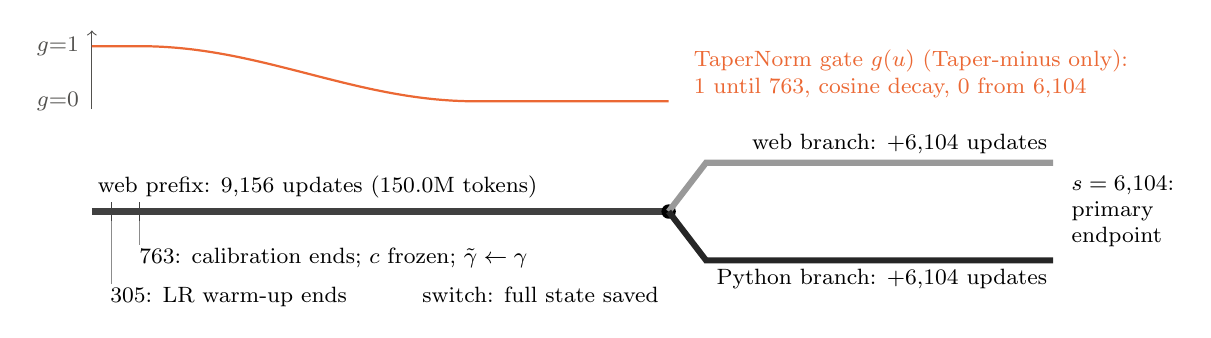
\begin{tikzpicture}[x=0.8cm, y=1cm, font=\footnotesize]
  % TaperNorm gate g(u), Taper-minus only
  \draw[inkmuted, ->] (0,1.3) -- (0,2.3);
  \node[inkmuted, anchor=east] at (-0.05,2.1) {$g{=}1$};
  \node[inkmuted, anchor=east] at (-0.05,1.4) {$g{=}0$};
  \draw[taperorange, thick] (0,2.1) -- (0.763,2.1) -- plot[domain=0.763:6.104, samples=60]
        (\x, {1.4 + 0.7*0.5*(1+cos(180*(\x-0.763)/5.341))}) -- (9.156,1.4);
  \node[taperorange, anchor=west, align=left] at (9.4,1.75) {TaperNorm gate $g(u)$ (Taper-minus only):\\1 until 763, cosine decay, 0 from 6{,}104};
  % prefix
  \draw[line width=2.2pt, black!75] (0,0) -- (9.156,0);
  \node[anchor=south west, inner sep=2pt] at (0,0.1) {web prefix: 9{,}156 updates (150.0M tokens)};
  \foreach \u in {0.305, 0.763} { \draw[black!75] (\u,-0.12) -- (\u,0.12); }
  \draw[black!45] (0.763,-0.12) -- (0.763,-0.42);
  \node[anchor=north west, inner sep=1pt] at (0.70,-0.42) {763: calibration ends; $c$ frozen; $\tilde\gamma \leftarrow \gamma$};
  \draw[black!45] (0.305,-0.12) -- (0.305,-0.92);
  \node[anchor=north west, inner sep=1pt] at (0.24,-0.92) {305: LR warm-up ends};
  % switch and branches
  \fill (9.156,0) circle (2.6pt);
  \node[anchor=north east, inner sep=1pt] at (9.05,-0.92) {switch: full state saved};
  \draw[line width=2.2pt, black!40] (9.156,0) -- (9.75,0.62) -- (15.26,0.62);
  \draw[line width=2.2pt, black!85] (9.156,0) -- (9.75,-0.62) -- (15.26,-0.62);
  \node[anchor=south east, inner sep=2pt] at (15.26,0.66) {web branch: +6{,}104 updates};
  \node[anchor=north east, inner sep=2pt] at (15.26,-0.66) {Python branch: +6{,}104 updates};
  \node[anchor=west, align=left] at (15.4,0) {$s = 6{,}104$:\\primary\\endpoint};
\end{tikzpicture}
\caption{One condition and seed of the design. Both conditions start from identical initial weights and read the
same data order for each seed. At the switch, each condition's complete state (weights, optimizer moments, loss
scale and random-number state) is saved, and both of its branches restore that identical state. The web branch
continues on C4; the Python branch trains on Python files from The Stack. The global learning-rate clock continues through the branches without a restart.
Evaluations follow the schedule in \cref{app:schedule}.}
\label{fig:design}
\end{figure}

\paragraph{Optimization.} The optimizer is AdamW \citep{loshchilov2019adamw} with $\beta = (0.9, 0.95)$ and
$\epsilon = 10^{-8}$. All two-dimensional parameters, embeddings included, get weight decay $0.1$; gain vectors
get none. Gradients are clipped once per update to global norm $1.0$, after accumulation. Each update uses
$32 \times 512 = 16{,}384$ supervised tokens. The learning rate rises linearly to $6\times10^{-4}$ over 305
updates and then follows a cosine decay to $6\times10^{-5}$ at global update 15{,}260. The branches continue this
global clock, with no learning-rate restart, optimizer reset, replay or regularization toward the prefix
(\cref{fig:design}).

\paragraph{Pairing.} Seeds 101, 102 and 103 are paired across conditions. A canonical RMS initialization is
generated from the seed and explicitly copied into the Taper-minus model; $\tilde\gamma$ starts at~1 and is
inactive until update 764. Both conditions read the same pre-generated window order. Each run consists of a
prefix of 9{,}156 updates (150{,}011{,}904 tokens) followed by two branches of 6{,}104 updates each
(100{,}007{,}936 tokens). The web branch reads further unseen web windows and the Python branch reads Python
windows; no window repeats within a trajectory. The primary allocation is 2.10B supervised tokens.

\paragraph{Precision.} Training ran in FP16 autocast with dynamic loss scaling \citep{micikevicius2018mixed}.
Master weights, optimizer moments, normalization and calibration statistics, and the loss were kept in FP32.
A step whose gradients were nonfinite was to be retried on the same batch at a halved loss scale, so no update
is ever skipped. This replaced the protocol's original BF16 plan, because the available hardware (NVIDIA T4)
lacks efficient BF16 support (\cref{tab:amendments}).

\subsection{Data}

\paragraph{Sources.} Web text comes from C4 English \citep{raffel2020t5} (revision \texttt{\cfourRev}); training
uses the official training split, and the official validation split is hashed 50/50 into development and
reserved-test sets. Code comes from the Python subset of The Stack (deduplicated) \citep{kocetkov2022stack}
(revision \texttt{\stackRev}). Files are grouped into connected components over their repository-name aliases
(\repoGroups{} groups), and each group is assigned by $\mathrm{sha256}(\text{group}) \bmod 100$: 0--89 train,
90--94 development, 95--99 test.

\paragraph{Deduplication.} Documents are deduplicated exactly by content hash across all domains and splits. An
approximate near-duplicate audit uses MinHash \citep{broder1997resemblance} over GPT-2 token 5-grams (128
permutations, LSH with 32 bands of 4 rows), confirmed by exact Jaccard similarity $\ge 0.85$. When duplicates
straddle splits, the copy in the higher-priority split is kept (test over development over training). This removed \exactRemoved{} exact and \nearRemoved{} near duplicates.

\paragraph{Packing and quotas.} Text is tokenized with GPT-2 BPE, with one EOS appended per document, and packed
into 513-token windows at stride 512 with no padding. Quotas are \webTrainTokens{} web and \pyTrainTokens{} Python
training tokens, and 2{,}097{,}152 development labels (4{,}096 windows) per domain. The \emph{quick} development
set is the first 262{,}144 of those labels. Reserved-test sets of 8{,}388{,}608 labels per domain were sealed and
never used. The non-whitespace code CE used to measure adaptation excludes class W only.

\subsection{Evaluation schedule and decision rules}

Full development evaluations ran at 13 prefix points and at 25 continuation points per branch. Quick
development evaluations ran at the switch and at 80 continuation points per branch, dense early on (\cref{app:schedule}). Every full
evaluation stores per-document and per-class sufficient statistics.

The secondary \emph{matched-adaptation} analysis is fixed in advance. It fixes targets at the RMS Python branch's
quick-dev code CE at $s \in \{1525, 3050, 6104\}$. It finds the first downward crossing of each target by
Taper-minus within an observed bracket of at most 100 updates (no extrapolation) and interpolates Taper-minus's
web CE at that crossing. It then compares the two models' web forgetting relative to their own $s = 0$.

The decision rules in \cref{tab:rules} are applied in order once all three seed groups are complete. They are
screening criteria, not significance tests. With three seeds, the reported 95\% interval
$\bar D \pm 4.303\, s_D/\sqrt{3}$ is descriptive.

\begin{table}[t]
\centering
\small
\caption{Pre-specified decision rules, applied in order. CE values are in nats/token; a bar denotes the mean over
seeds.}
\label{tab:rules}
\begin{tabular}{@{}clp{8.6cm}@{}}
\toprule
\# & Category & Condition \\
\midrule
1 & Invalid or incomplete & Missing seed group, unresolved correctness or data failure, nonfinite primary run, or resource termination \\
2 & Comparability / adaptation limited & Any seed's relative prefix web-CE gap $> 2\%$, or either condition's Python branch improves non-W code CE by $< 0.05$ \\
3 & Opposite direction & $\bar D \le -0.03$ \\
4 & Proceed to design next study & $\bar D \ge 0.03$; $D > 0$ in every seed; $\bar D(3050) \ge 0.015$; $\bar Q > 0.5\,\bar D$; mean matched differential forgetting $> 0$ at the furthest common target \\
5 & Transient only & $\bar D < 0.015$ and quick-dev $\bar D(s) \ge 0.05$ at some scheduled $s \le 1000$ \\
6 & Stop: small observed effect & $\bar D < 0.015$ \\
7 & Inconclusive & Anything else \\
\bottomrule
\end{tabular}
\end{table}

\subsection{Pre-specification and amendments}
\label{sec:prespec}

The hypothesis, design, estimands, evaluation schedule and decision thresholds come from a written protocol
(``protocol v3''), drafted before the data were prepared. \authornote{Confirm the protocol's drafting date
(the project export suggests 11--12 September 2026) and where it was kept.} The protocol was not lodged with an
external registry, which is a limitation (\cref{sec:limitations}). The amendments in \cref{tab:amendments} were
made before any primary-run update; none of them changes the model, data, token budgets, seeds, endpoint or
thresholds.

The primary run's configuration (thresholds, schedule, batch layout and data hashes) was frozen into a hash
(\texttt{\configSha\ldots}) at launch, and the analysis is a deterministic function of the stored evaluation
records. A public commit containing the protocol and the analysis code was made on 2026-10-03 at 16:07~UTC: after
the primary run had started (\sessionStart{}~UTC) but before it finished (\sessionEnd{}~UTC).

Before the primary run, engineering runs measured throughput and verified checkpoint resume. These included
earlier preflights under a separate engineering seed, and a 25-minute smoke test that repeated roughly the first
2{,}300 prefix updates of seed 101 for both conditions. These runs were discarded. None of them reached the switch,
so no continuation-phase quantity, and hence no value of $D$, was computed before the primary run.
\authornote{Confirm that no earlier run (including exploratory runs on proxy corpora) produced a $D$-like
contrast on these data.}

\begin{table}[t]
\centering
\small
\caption{Protocol amendments, all made before the primary run.}
\label{tab:amendments}
\begin{tabular}{@{}lp{12.2cm}@{}}
\toprule
Date & Amendment \\
\midrule
2026-09-28 & NVIDIA T4 hardware: FP16 autocast with dynamic loss scaling replaces BF16; FP32 master weights, moments, normalization and EMA statistics, and loss. Results are not pooled with any BF16 run. \\
2026-09-30 & Free cloud GPU time spread over sessions replaces the original 24-GPU-hour paid budget; the scientific allocation is unchanged. \\
2026-10-01 & RMS and Taper-minus are trained as independent processes on two GPUs, with no shared state. \\
2026-10-03 & Microbatch of 8 sequences $\times$ 4 accumulation steps (the protocol's default layout; effective batch unchanged). For storage, model weights are kept only for the switch state and branch endpoints; the per-document and per-class statistics required at every full-development point are kept. \\
\bottomrule
\end{tabular}
\end{table}

\section{Execution and implementation checks}
\label{sec:execution}

The primary run took one \sessionHours-hour session on a cloud machine with two NVIDIA Tesla T4 GPUs (PyTorch
\torchVersion, CUDA \cudaVersion), with RMS on one GPU and Taper-minus on the other. All six condition--seed runs
completed all 21{,}364 updates. There were no nonfinite losses, gradients or weights, and the loss scale never
needed a retry (\overflowRetries{} retries in total). Gradient clipping was active in \clipRMSlo--\clipRMShi\% of
updates for RMS and \clipTaperlo--\clipTaperhi\% for Taper-minus. GPU kernels used for the backward pass are
nondeterministic, so results are reproducible to within numerical noise, not bitwise.

The training code is a single script that transcribes a separately tested reference implementation of the model,
optimizer step and analysis. Before the run, it was checked against that reference in seven ways:
\begin{enumerate}[label=(\roman*),leftmargin=1.8em,itemsep=1pt]
  \item identical learning-rate and gate values at all 15{,}260 updates;
  \item identical paired initial tensors;
  \item FP32 training updates during the calibration phase that match the reference update to a relative
        tolerance of $2\times10^{-5}$;
  \item bit-identical FP32 model outputs at updates spanning every TaperNorm gate state;
  \item a vectorized evaluator that reproduces the reference evaluator's CE and class sums on the real
        development data, to a relative tolerance of $10^{-9}$;
  \item identical decision categories on 3{,}000 randomly generated evidence sets;
  \item checkpoint resume whose deviation from an uninterrupted run is of the same order as run-to-run GPU
        nondeterminism.
\end{enumerate}
The primary contrasts in \cref{sec:results} were also recomputed independently from the raw evaluation records,
and they agree with the frozen analysis output.

\section{Results}
\label{sec:results}

\subsection{Validity checks}

\Cref{tab:validity} shows that every guardrail passed.
\begin{itemize}[leftmargin=1.4em,itemsep=2pt]
  \item \textbf{Comparable prefixes.} The relative gap in prefix web CE was \gapMin--\gapMax\% (limit 2\%),
        with Taper-minus slightly lower in every seed. Over the last five prefix evaluations, both conditions were
        still improving at nearly the same rate (mean slope \slopeRMS{} vs.\ \slopeTaper{} nats per million
        tokens).
  \item \textbf{Strong adaptation.} Both conditions adapted strongly to Python: non-W code CE fell by
        \adaptMin--\adaptMax{} nats (minimum 0.05), and the adaptation curves almost coincide
        (\cref{fig:trajectories}c).
  \item \textbf{Large forgetting in both conditions.} The Python branch raised web CE by \FcodeMin{} to
        \FcodeMax{} nats/token relative to the switch, while web continuation lowered it by 0.12--0.13
        (\cref{fig:trajectories}a).
\end{itemize}

\begin{table}[t]
\centering
\small
\caption{Validity checks and actual forgetting $F$ (full-dev web CE, nats/token). ``Gap'' is the absolute prefix
web-CE difference relative to RMS (limit 2\%). ``Code gain'' is the Python branch's reduction in non-W code CE
from the switch to $s = 6{,}104$ (minimum 0.05).}
\label{tab:validity}
\begin{tabular}{@{}lrrrrrrrr@{}}
\toprule
 & \multicolumn{2}{c}{Prefix web CE} & & \multicolumn{2}{c}{$F$, web branch} & \multicolumn{2}{c}{$F$, Python branch} & \\
\cmidrule(lr){2-3}\cmidrule(lr){5-6}\cmidrule(lr){7-8}
Seed & RMS & Taper & Gap & RMS & Taper & RMS & Taper & Code gain (R / T) \\
\midrule
101 & $4.5846$ & $4.5716$ & $0.28\%$ & $-0.128$ & $-0.128$ & ${+}1.655$ & ${+}1.636$ & $3.55$ / $3.55$ \\
102 & $4.5795$ & $4.5666$ & $0.28\%$ & $-0.123$ & $-0.122$ & ${+}1.688$ & ${+}1.668$ & $3.60$ / $3.46$ \\
103 & $4.5931$ & $4.5773$ & $0.34\%$ & $-0.128$ & $-0.124$ & ${+}1.655$ & ${+}1.633$ & $3.35$ / $3.34$ \\
\bottomrule
\end{tabular}

\end{table}

\subsection{Primary endpoint}

\begin{table}[t]
\centering
\small
\caption{Primary contrast $D$ at $s = 6{,}104$ and secondary contrasts (nats/token; full development set). Positive
values mean more excess web forgetting for Taper-minus. ``Matched'' is the matched-adaptation differential
forgetting at the furthest target reached by every seed ($s = \matchedTarget$).}
\label{tab:primary}
\begin{tabular}{@{}lrrrrrr@{}}
\toprule
Seed & $D$ & $D(3050)$ & $D(1525)$ & $G_{\text{web}}$ & $Q$ & Matched ($s{=}6104$) \\
\midrule
101 & $-0.0200$ & ${+}0.0109$ & ${+}0.0369$ & $-0.0006$ & $-0.0194$ & $-0.0308$ \\
102 & $-0.0207$ & $-0.0124$ & ${+}0.0224$ & $-0.0009$ & $-0.0199$ & $-0.0182$ \\
103 & $-0.0262$ & ${+}0.0193$ & $-0.0286$ & $-0.0042$ & $-0.0220$ & $-0.0286$ \\
\midrule
Mean & $-0.0223$ & ${+}0.0059$ & ${+}0.0102$ & $-0.0019$ & $-0.0204$ & $-0.0259$ \\
SD & $0.0034$ & $0.0165$ & $0.0344$ & $0.0020$ & $0.0014$ & $0.0067$ \\
\bottomrule
\end{tabular}

\end{table}

\Cref{tab:primary} gives the primary results. Mean $D$ = \Dmean{}~nats/token (SD \Dsd; descriptive 95\% interval
$[\Dlo, \Dhi]$), and $D$ is negative in all three seeds. Since $\bar D < 0.015$ and no early transient reached
0.05 (below), the pre-specified decision is \textbf{stop: small observed effect} (rule~6). The data provide no
evidence for H1.

The other quantities point the same way as $D$:
\begin{itemize}[leftmargin=1.4em,itemsep=2pt]
  \item $G_{\text{web}}$ is close to zero (mean \Gmean), so the difference sits in the Python branch itself: the
        direct differential forgetting $Q$ averages \Qmean.
  \item The matched-adaptation contrast at $s = \matchedTarget$ averages \matchedMean{}, negative in every seed.
        On the quick development set, Taper-minus reached the RMS code-CE target before the corresponding RMS
        update in \matchedEarlier{} of \matchedPairs{} seed--target pairs (\cref{app:extra}). At the furthest
        target, then, Taper-minus also showed slightly less web forgetting when compared at matched code
        adaptation.
  \item The per-document and per-class decompositions reconstruct $D$ exactly. The effect is broad rather than
        driven by a few documents: median per-document $D_i$ lies between \medianDocMin{} and \medianDocMax{}.
        By token class, alphanumeric tokens contribute negatively in all \classAneg{} seeds and give the largest
        share in \classAlargest{} of them; in seed 101, punctuation and symbol tokens contribute more
        (\cref{app:extra}).
\end{itemize}

\subsection{Size and stability of the difference}

\begin{figure}[t]
\centering
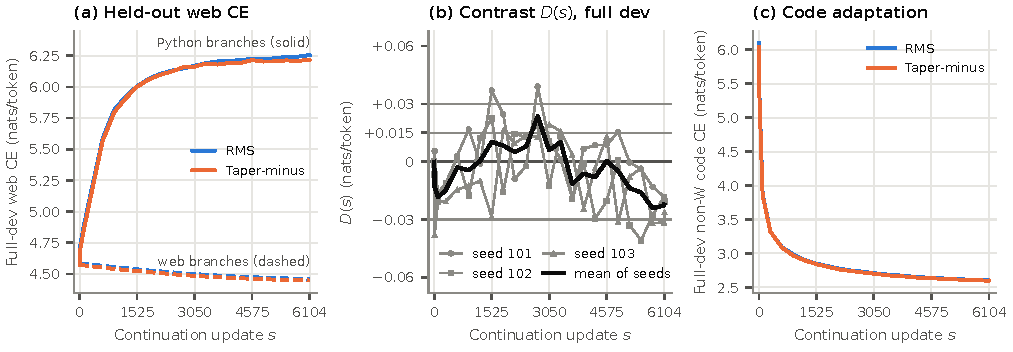
\includegraphics[width=\linewidth]{figures/trajectories.pdf}
\caption{Continuation trajectories on the full development sets (means over three seeds unless stated).
\textbf{(a)} Held-out web CE in all four branches. RMS and Taper-minus nearly coincide within each branch, and the
Python branches show large forgetting. \textbf{(b)} The contrast $D(s)$ for each seed and their mean. The labelled
horizontal lines are the pre-specified thresholds ($+0.03$ proceed, $+0.015$ small-effect bound, $-0.03$ opposite
direction); the decision uses only $s = 6{,}104$ (and $s = 3{,}050$ for rule~4). \textbf{(c)} Non-whitespace code CE on
the Python branch, showing near-identical adaptation in the two conditions.}
\label{fig:trajectories}
\end{figure}

The difference between the conditions is small in absolute terms: $|\bar D|$ is \DrelPct\% of the mean Python-branch
forgetting, which is \FcodeMean{} nats/token. Its sign was also not stable during continuation
(\cref{fig:trajectories}b):
\begin{itemize}[leftmargin=1.4em,itemsep=2pt]
  \item A single seed's $D(s)$ changed by up to \maxJump{} between neighbouring full evaluations, and the
        largest $|D(s)|$ of any seed was \seedAbsMax.
  \item The seed-mean $D(s)$ ranged from \trajMin{} at $s = \trajMinAt$ to \trajMax{} at $s = \trajMaxAt$.
  \item At $s = 1{,}525$ the seeds gave \DoneFiveA, \DoneFiveB{} and \DoneFiveC; at $s = 3{,}050$ the mean was
        \DthreeMean, with mixed signs.
\end{itemize}
The quick-dev contrast never approached the transient threshold: its seed mean peaked at \earlyMax{} (at
$s = \earlyMaxAt$) within the first 1{,}000 updates, against a threshold of 0.05.

The consistently negative endpoint is therefore one value from a fluctuating trajectory. It was pre-specified
precisely so that no favourable checkpoint could be chosen afterwards.

\section{Discussion}

\paragraph{What the result shows.} In this setting, replacing internal RMSNorm with TaperNorm did not increase
persistent forgetting of web text after a switch to Python. The pre-specified screen for a meaningful excess
($\bar D \ge 0.015$) was not met, and every seed's endpoint $D$ was below zero. Under the protocol's rules this direction is stopped. No seeds were
added, no endpoint was changed and no follow-up was launched.

\paragraph{What it does not show.} \emph{Stop} is not evidence of equivalence \citep{lakens2017equivalence}, and
the negative endpoint is not evidence that TaperNorm protects against forgetting. That effect would have needed
$\bar D \le -0.03$, which was not reached. The intermediate-checkpoint fluctuations in \cref{fig:trajectories}b
are as large as the endpoint value, and three seeds give a fragile estimate of seed-to-seed variance
\citep{dodge2020finetuning}. The descriptive interval is conditional on one prepared corpus sample and one
training recipe; it is not a population bound.

\paragraph{Why the concern may not have materialized (conjecture).} We did not test mechanisms, but three
features of the setting may matter.
\begin{itemize}[leftmargin=1.4em,itemsep=2pt]
  \item Taper-minus keeps the final RMSNorm, which \citet{kanavalau2026tapernorm} identify as the essential scale
        anchor.
  \item $\tilde\gamma$ and all weight matrices remain trainable after the taper, so scale changes can be absorbed
        cheaply.
  \item The forgetting here is very large in both conditions, which suggests that most of it comes from factors
        the two architectures share.
\end{itemize}
Each of these is a hypothesis for a future study, not a finding of this one.

\section{Limitations}
\label{sec:limitations}

\begin{itemize}[leftmargin=1.4em,itemsep=2pt]
  \item \textbf{Scale.} The models have \paramsRMS{} parameters, about \embedShare\% of them in embeddings, and see
        150M prefix tokens. Embedding drift may mediate or interact with the condition effect, and results may
        not transfer to larger models or longer training.
  \item \textbf{Breadth.} There is one domain pair (web to Python), one data sample, one optimizer recipe and one
        hardware and precision setting (FP16 on T4, not the protocol's original BF16). The auxiliary-loss variant
        of TaperNorm (Taper-plus) was not run.
  \item \textbf{Statistics.} Three paired seeds share one prepared corpus, so uncertainty is conditional on that
        corpus, and the interval in \cref{tab:primary} is descriptive. All measurements use development data; the
        reserved test sets remain sealed for any confirmatory study.
  \item \textbf{Pre-specification.} The protocol was kept privately and not registered externally. The public
        record of the analysis code postdates the start of the primary run (\cref{sec:prespec}).
  \item \textbf{Data audit.} The near-duplicate search is approximate, and the random audit of \auditPairs{}
        cross-split document pairs (\auditFound{} found above threshold) has low power to detect rare leakage.
        Repository names are an incomplete proxy for forks.
  \item \textbf{Secondary analyses.} Matched adaptation interpolates between evaluated checkpoints and describes
        curves; it does not evaluate an actual model. Activation and attention diagnostics were logged but are
        not analysed here.
\end{itemize}

\section{Conclusion}

A small pilot, specified before training, found no evidence that TaperNorm increases persistent forgetting after
a web-to-code domain shift: mean $D$ = \Dmean{}~nats/token, against a pre-specified $+0.015$ bound. The
difference pointed the other way at the endpoint, but it was small and unstable across checkpoints, so we draw
no conclusion about protection. Testing H1 more broadly would need a new pre-specified study with larger models,
more seeds and more than one domain shift. On its own, this pilot does not justify one.

\section*{Code and data availability}
The code (data preparation, training, evaluation and the frozen analysis), the frozen configuration with data and
source hashes, the decision report, and every evaluation record behind the tables and figures are available at
\authornote{repository URL, currently \url{https://github.com/Danieldotcomcoder/domain-shift-forgettting}}.
The script \texttt{paper/make\_assets.py} regenerates every number, table and figure in this paper from those
records. C4 and The Stack are subject to their own licenses and terms of use; no corpus text is redistributed.

\section*{Acknowledgements}
\authornote{Disclose AI assistance as required by arXiv policy, for example: ``The training and analysis code
and a first draft of this manuscript were prepared with assistance from an AI system (Claude, Anthropic). The
author designed the study, reviewed all code and text, and takes full responsibility for the content.'' Adjust
this to reflect your actual roles.}

\bibliographystyle{plainnat}
\bibliography{refs}

\clearpage
\appendix

\section{Evaluation schedule}
\label{app:schedule}

\paragraph{Full development evaluations (2{,}097{,}152 labels per domain).} Prefix: global updates 763, 3052,
6104, 6409, 6714, 7019, 7324, 7629, 7934, 8239, 8544, 8849 and 9156. Continuation (each branch):
$s \in \{0, 1, 10, 100\}$, every 305 updates from 305 to 6100, and 6104.

\paragraph{Quick development evaluations (262{,}144 labels per domain).} At the switch, and at continuation
$s \in \{0, 1, 2, 5, 10, 20\}$, every 50 updates from 50 to 1000, every 100 updates from 1100 to 6100, and
$\{1525, 3050, 6104\}$ (80 points). Quick-dev values describe transients and feed matched adaptation. They never
enter the full-dev primary contrast.

\paragraph{Diagnostics.} Forward-only activation, gain and attention-entropy probes on the last 256 training
windows of each domain, at the switch and at $s \in \{0, 10, 100, 1525, 6104\}$. They are logged but not analysed
here.

\section{Additional results}
\label{app:extra}

\begin{table}[H]
\centering
\small
\caption{Matched-adaptation differential forgetting (nats/token) and the interpolated Taper-minus update at which
it reached each RMS code-CE target, with the observed bracket in parentheses.}
\begin{tabular}{@{}lrrrrrr@{}}
\toprule
 & \multicolumn{3}{c}{Matched differential forgetting} & \multicolumn{3}{c}{Taper update at match (bracket)} \\
\cmidrule(lr){2-4}\cmidrule(lr){5-7}
Seed & $s{=}1525$ & $s{=}3050$ & $s{=}6104$ & $s{=}1525$ & $s{=}3050$ & $s{=}6104$ \\
\midrule
101 & $-0.0075$ & $-0.0038$ & $-0.0308$ & 1447 (1400--1500) & 2740 (2700--2800) & 5198 (5100--5200) \\
102 & ${+}0.0094$ & $-0.0106$ & $-0.0182$ & 1475 (1400--1500) & 2776 (2700--2800) & 5775 (5700--5800) \\
103 & $-0.0259$ & ${+}0.0145$ & $-0.0286$ & 1519 (1500--1525) & 3024 (3000--3050) & 5862 (5800--5900) \\
\bottomrule
\end{tabular}

\end{table}

\begin{table}[H]
\centering
\small
\caption{Decomposition of the endpoint $D$ (nats/token) into disjoint token classes (each class's contribution
weighted by its label share; the four contributions sum to $D$), and summaries of per-document effects $D_i$ over
the \nDocsWeb{} web development documents. ``Top-1\% sum'' is the signed contribution of the 1\% of documents
with the largest positive contributions.}
\begin{tabular}{@{}lrrrrrrr@{}}
\toprule
 & \multicolumn{4}{c}{Contribution to $D$ by token class} & \multicolumn{3}{c}{Per-document $D_i$} \\
\cmidrule(lr){2-5}\cmidrule(lr){6-8}
Seed & W & A & P & X & Median & 1\%-trimmed & Top-1\% sum \\
\midrule
101 & ${+}0.0038$ & $-0.0098$ & $-0.0121$ & $-0.0019$ & $-0.0232$ & $-0.0203$ & ${+}0.0018$ \\
102 & $-0.0019$ & $-0.0155$ & ${+}0.0014$ & $-0.0047$ & $-0.0257$ & $-0.0210$ & ${+}0.0020$ \\
103 & ${+}0.0008$ & $-0.0227$ & $-0.0055$ & ${+}0.0012$ & $-0.0272$ & $-0.0265$ & ${+}0.0020$ \\
Labels & 33,807 & 1,786,076 & 230,998 & 46,271 & \multicolumn{3}{c}{4,409 documents} \\
\bottomrule
\end{tabular}

\end{table}

\end{document}
